\subsection{Systemsekvensdiagram(SSD)}

Herefter begynder artefakterne at komme tættere på koden.
Ud fra Use Casesene opbygget i afsnit \ref{UseCases} kan vi oprette et SSD for hver use case.

Et SSD viser, hvordan en bruger vil tale sammen med systemet.
Det er vigtigt, at systemet skal holdes som en sort kasse, da dette diagram udelukkende har med brugeren og systemet at gøre.

Diagrammet kan bruges til at blive enig med PO om, hvordan de ønsker at kunne tale med systemet uden at diskutere noget teknisk, som kan skabe unødvendig forvirring.

Det kan skabe problemer, hvis man begynder at bekymre sig om, hvordan systemet arbejder med brugerens input ved udarbejdelsen af et SSD.
Man risikerer, at man kommer til at designe et system, som ikke opfører sig som brugeren ønsker, men er designet, så det er nemmest at implementere.

Et SSD kombineres så med en eller flere systemoperationskontrakter(SOC), til at konkretisere hvilke ændringer i systemet en interaktion mellem bruger og system giver anledning til.

På figur \ref{forretning:ssd} kan SSD'en for use casen 'book ny aftale' ses.
Bemærk, at dette artefakt og de næste artefakter vil være på engelsk.
Se afsnit \ref{glossary} for en ordliste.
Dette SSD viser, hvordan en bruger skal tale med systemet, når brugeren ønsker at booke en ny aftale.

\begin{figure}[H]
    \caption{SSD for Book Ny Aftale}
    \centering
        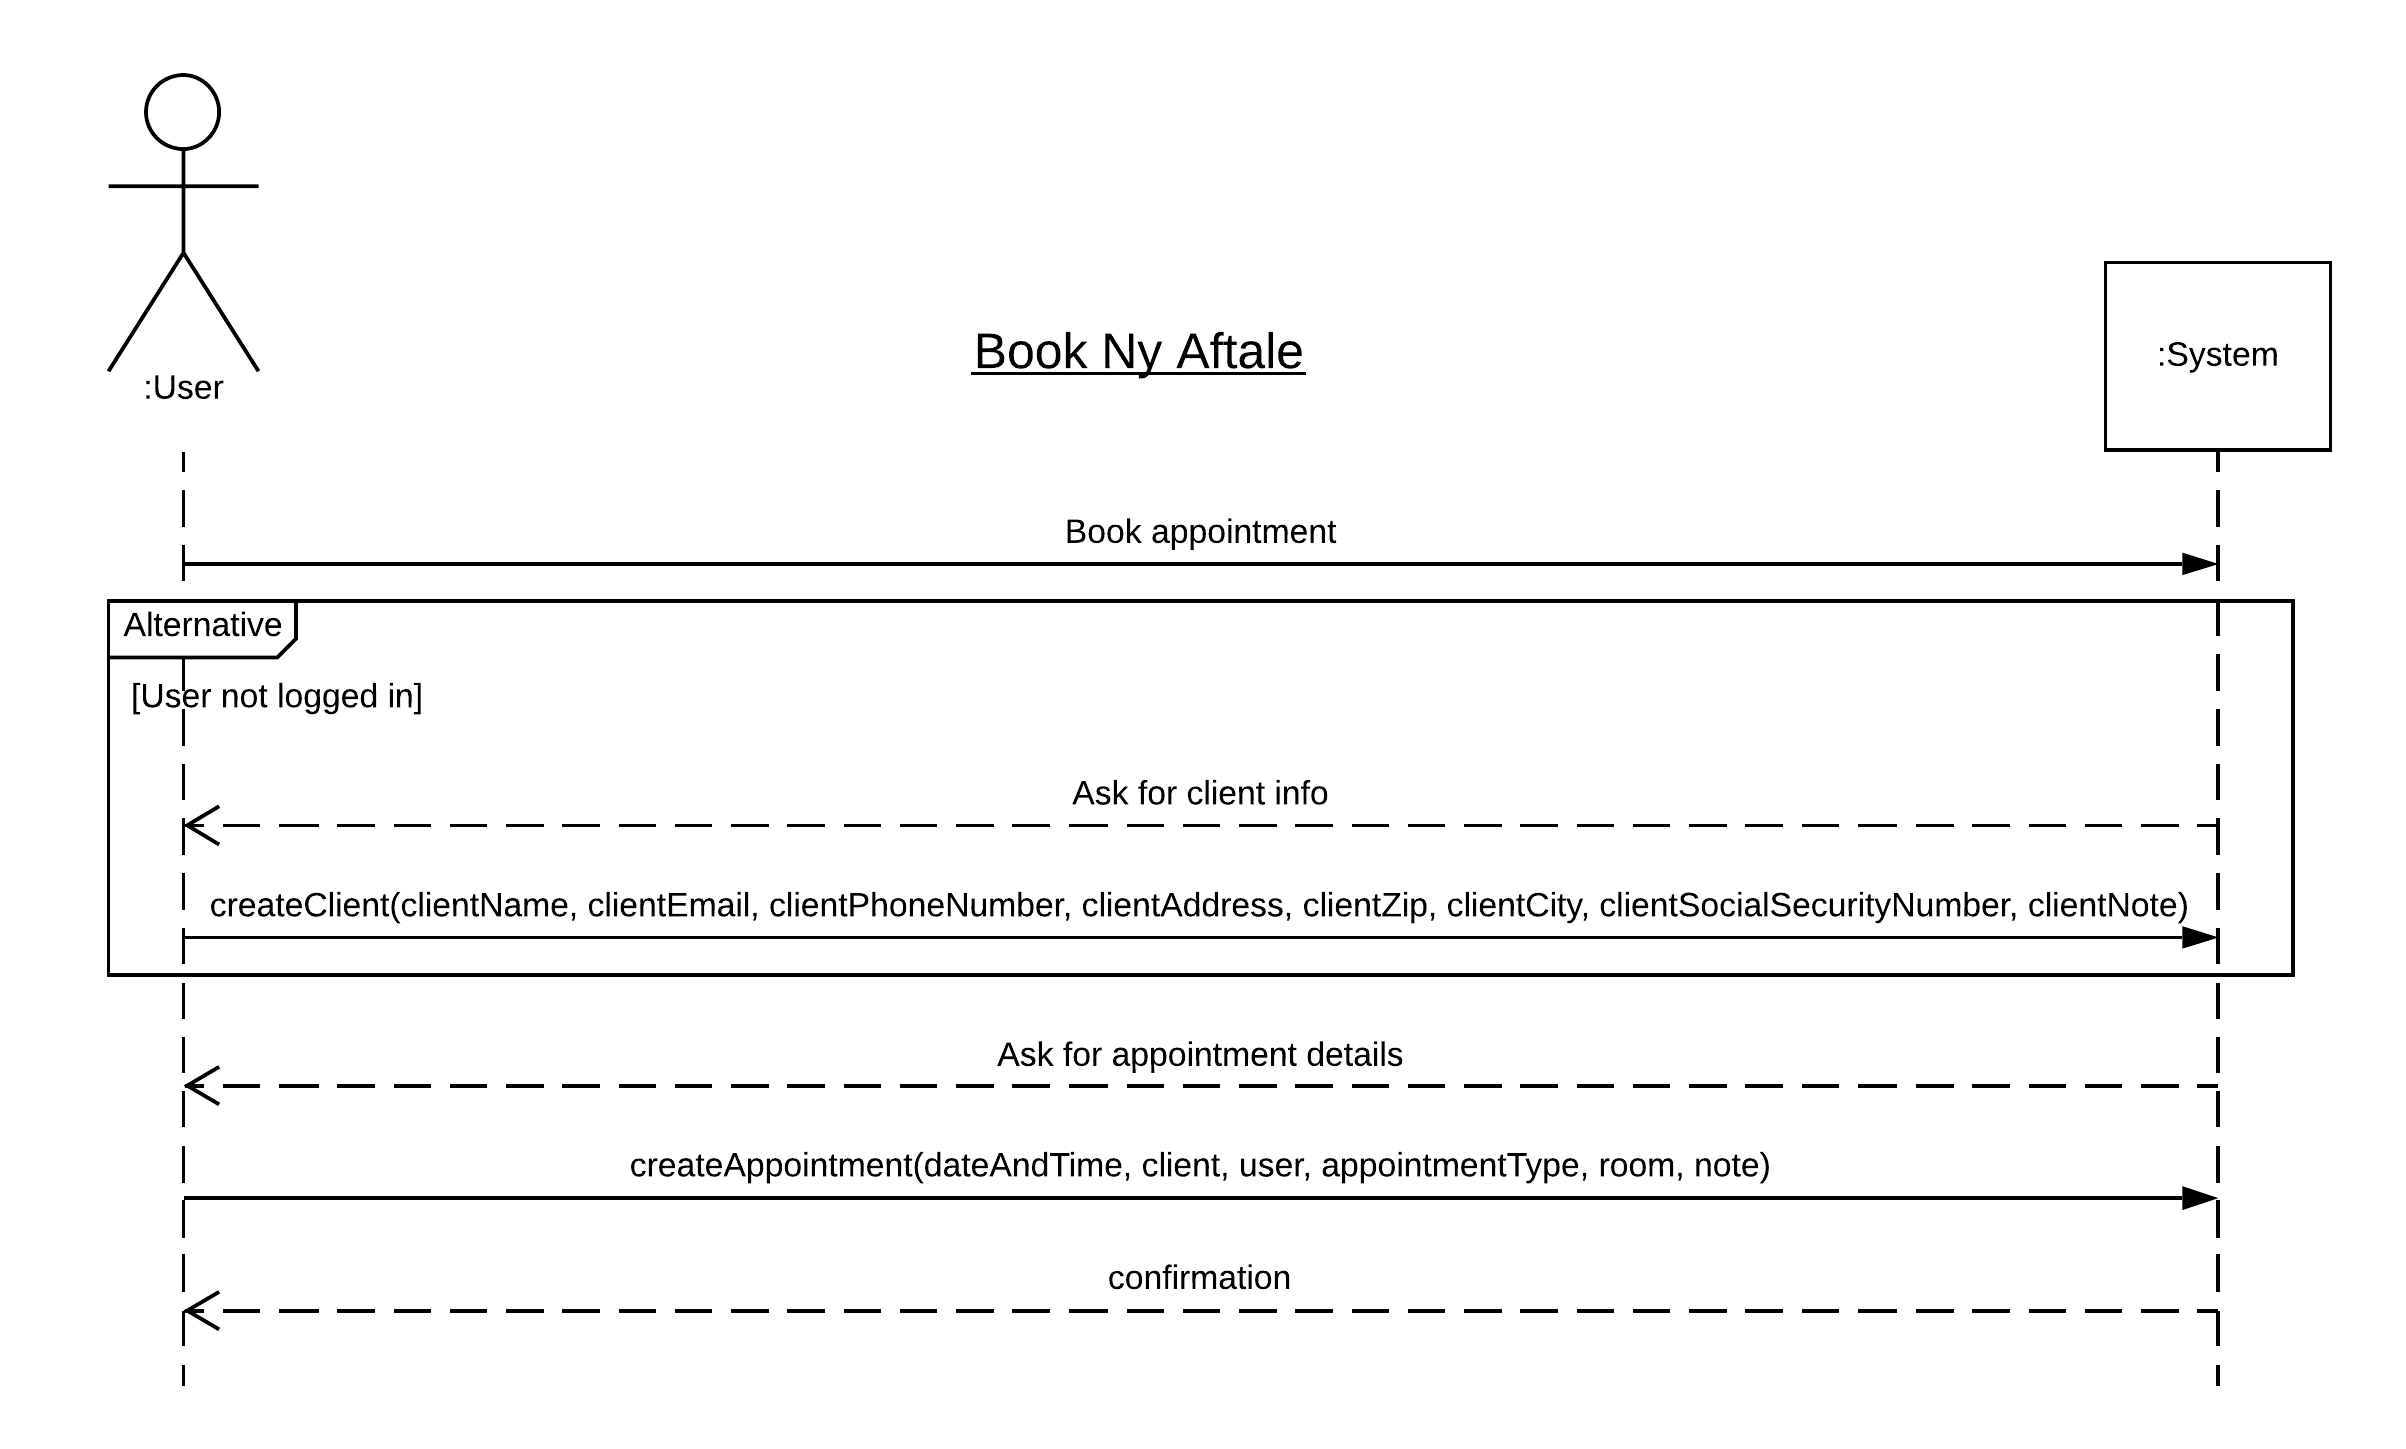
\includegraphics[width=\textwidth]{SSD.png}
    \label{forretning:ssd}
\end{figure}
